
\begin{figure}[h]
        \begin{minipage}{0.24\textwidth}
            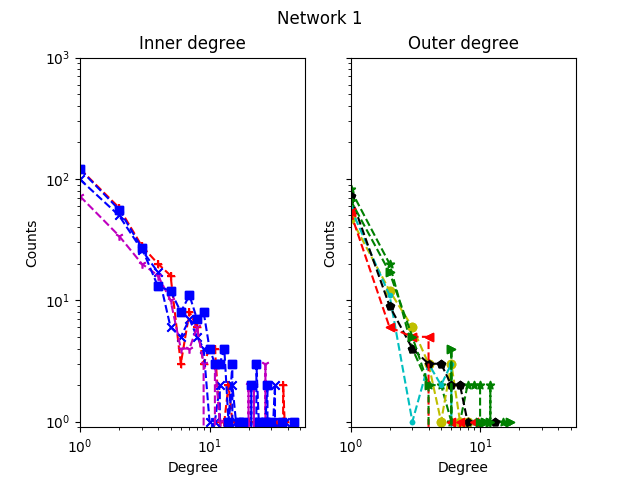
\includegraphics[width=\textwidth]{img/corpus/network1_1}
        \end{minipage}
        \begin{minipage}{0.24\textwidth}
            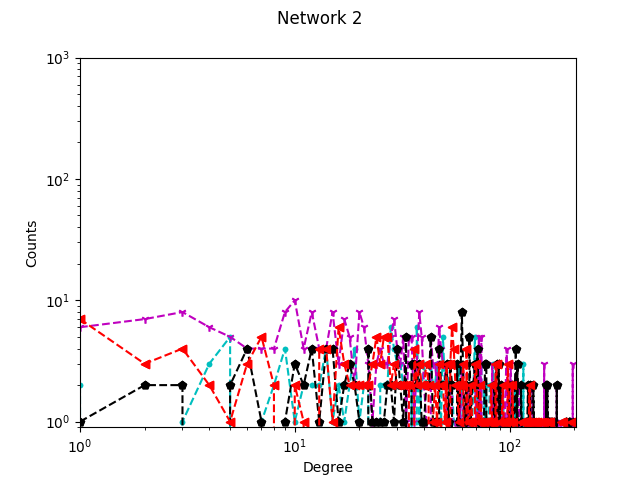
\includegraphics[width=\textwidth]{img/corpus/network2_1}
        \end{minipage}
        \vskip\baselineskip
        \begin{minipage}{0.24\textwidth}
            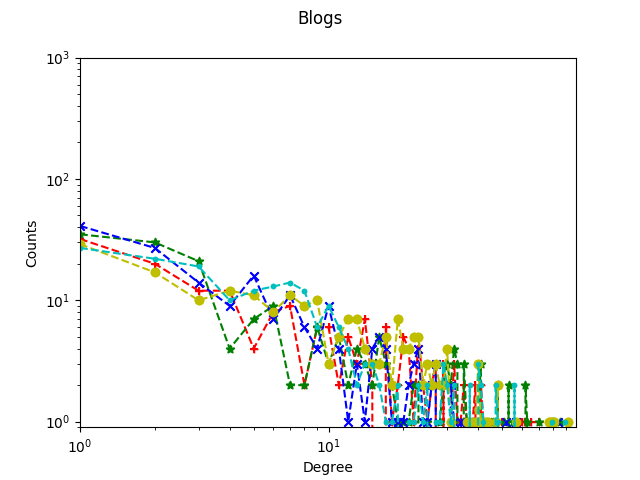
\includegraphics[width=\textwidth]{img/corpus/blogs_1}
        \end{minipage}
        \begin{minipage}{0.24\textwidth}
            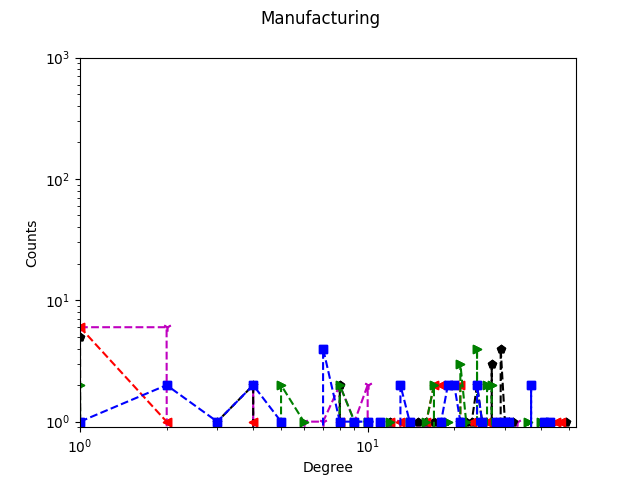
\includegraphics[width=\textwidth]{img/corpus/manufacturing_1}
        \end{minipage}
        \caption {Local degree distributions for the four training datasets. For Network1 and Network2 the classes come from ground-truth. For Blogs and Manufacturing we use classes find by a Louvain algorithms.} 
	\label{fig:synt_graph_local}
\end{figure}
